\documentclass[a4paper]{article}
\addtolength{\hoffset}{-2.25cm}
\addtolength{\textwidth}{4.5cm}
\addtolength{\voffset}{-3.25cm}
\addtolength{\textheight}{5cm}
\setlength{\parskip}{0pt}
\setlength{\parindent}{0in}

%----------------------------------------------------------------------------------------
%	PACKAGES AND OTHER DOCUMENT CONFIGURATIONS
%----------------------------------------------------------------------------------------

\usepackage{blindtext} % Package to generate dummy text
\usepackage{charter} % Use the Charter font
\usepackage[utf8]{inputenc} % Use UTF-8 encoding
\usepackage{microtype} % Slightly tweak font spacing for aesthetics
\usepackage[english]{babel} % Language hyphenation and typographical rules
\usepackage[T1]{fontenc}
\usepackage{wrapfig, subcaption, setspace}
\usepackage[font=small, labelfont=bf]{caption}
\usepackage{lastpage} % Provide ref to the last page
\usepackage{indentfirst} % Consistent indentation
\usepackage{amsfonts, amssymb, amsmath, bm} % Mathematical typesetting
\usepackage{float} % Improved interface for floating objects
\usepackage[final, colorlinks = true, 
            linkcolor = black, 
            citecolor = black]{hyperref} % For hyperlinks in the PDF
\usepackage{graphicx, multicol} % Enhanced support for graphics
\usepackage{xcolor} % Driver-independent color extensions
\usepackage{marvosym, wasysym} % More symbols
\usepackage{rotating} % Rotation tools
\usepackage{censor} % Facilities for controlling restricted text
\usepackage{listings, style/lstlisting} % Environment for non-formatted code, !uses style file!
\usepackage{pseudocode} % Environment for specifying algorithms in a natural way
\usepackage{style/avm} % Environment for f-structures, !uses style file!
\usepackage{booktabs} % Enhances quality of tables
\usepackage{tikz-qtree} % Easy tree drawing tool
\tikzset{every tree node/.style={align=center,anchor=north},
         level distance=2cm} % Configuration for q-trees
\usepackage{style/btree} % Configuration for b-trees and b+-trees, !uses style file!
\usepackage[backend=biber,style=numeric,
            sorting=nyt]{biblatex} % Complete reimplementation of bibliographic facilities
\addbibresource{ref.bib}
\usepackage{csquotes} % Context sensitive quotation facilities
\usepackage[yyyymmdd]{datetime} % Uses YEAR-MONTH-DAY format for dates
\renewcommand{\dateseparator}{-} % Sets dateseparator to '-'
\usepackage{fancyhdr} % Headers and footers
\pagestyle{fancy} % All pages have headers and footers
\fancyhead{}\renewcommand{\headrulewidth}{0pt} % Blank out the default header
\fancyfoot[L]{} % Custom footer text
\fancyfoot[C]{} % Custom footer text
\fancyfoot[R]{\thepage} % Custom footer text
\newcommand{\note}[1]{\marginpar{\scriptsize \textcolor{red}{#1}}} % Enables comments in red on margin

%----------------------------------------------------------------------------------------

\begin{document}

%-------------------------------
%	TITLE SECTION
%-------------------------------

\fancyhead[C]{}
\hrule \medskip % Upper rule
\begin{minipage}{0.295\textwidth} 
\raggedright
\footnotesize
YUCHEN WU, ZHAOCONG YUAN\hfill\\   
1002060244, 1002352777\hfill\\
\end{minipage}
\begin{minipage}{0.4\textwidth} 
\centering 
\large 
Assignment 3\\ 
\normalsize 
AER1513 Fall, 2020\\ 
\end{minipage}
\begin{minipage}{0.295\textwidth} 
\raggedleft
\today\hfill\\
\end{minipage}
\medskip\hrule 
\bigskip

%-------------------------------
%	CONTENTS
%-------------------------------

\newcommand{\vect}[1]{\bm{\mathbf{#1}}}
\newcommand{\mat}[1]{\bm{\mathbf{#1}}}

\section*{Question 1} 

From Figures 3.6 and 3.7 (from the assignment) of the speed and sensor noise histograms, it can be observed that the fitted Gaussians are approximately zero-mean and capture much of the variance in the histograms, with the only exceptions in $v_l$ and $v_r$ errors where the histograms are slightly left-skewed from the fitted Gaussian mean. Nevertheless, using zero-mean Gaussian noises is reasonable. The variances $Q_k, R^j_k$ are
\begin{align*}
    \mat{Q}_k 
    &= \begin{bmatrix} 
        \sigma_{v_x}^2 & 0 & 0 & 0 & 0 & 0 \\ 
        0 & \sigma_{v_y}^2 & 0 & 0 & 0 & 0 \\ 
        0 & 0 & \sigma_{v_z}^2 & 0 & 0 & 0 \\ 
        0 & 0 & 0 & \sigma_{\omega_1}^2 & 0 & 0 \\ 
        0 & 0 & 0 & 0 & \sigma_{\omega_2}^2 & 0 \\ 
        0 & 0 & 0 & 0 & 0 & \sigma_{\omega_3}^2 
    \end{bmatrix} T_K^2 
    = \begin{bmatrix} 
        0.0026 & 0 & 0 & 0 & 0 & 0 \\ 
        0 & 0.0021 & 0 & 0 & 0 & 0 \\ 
        0 & 0 & 0.0008 & 0 & 0 & 0 \\ 
        0 & 0 & 0 & 0.0090 & 0 & 0 \\ 
        0 & 0 & 0 & 0 & 0.0170 & 0 \\ 
        0 & 0 & 0 & 0 & 0 & 0.1747 
    \end{bmatrix} T_K^2 \\ 
    %
    \mat{R}^j_k 
    &= \begin{bmatrix}
        \sigma_{u_l}^2 & 0 & 0 & 0 \\
        0 & \sigma_{v_l}^2 & 0 & 0 \\
        0 & 0 & \sigma_{u_r}^2 & 0 \\
        0 & 0 & 0 & \sigma_{v_r}^2
    \end{bmatrix} 
    = \begin{bmatrix}
        38.0046 & 0 & 0 & 0 \\
        0 & 129.8544 & 0 & 0 \\
        0 & 0 & 41.9633 & 0 \\
        0 & 0 & 0 & 132.5082
    \end{bmatrix}
\end{align*}



% As seen from Figure 2.5 in the assignment, all four sources of errors, i.e. range, bearing, translational speed and rotational speed errors, are clearly unimodal and have close-to-zero mean with a spread. Range error and translational speed error align well with the corresponding fitted Gaussian distributions. It looks like bearing error and rotational speed error have a lighter tail than the fitted Gaussian. Overall, the assumption of zero-mean Gaussian noise sounds reasonable. The standard deviation of each source of errors are given in the figure.
% \begin{eqnarray*}
%     \mat{Q}_k & = \begin{bmatrix} q^v_k & 0 \\ 0 & q^\omega_k \end{bmatrix} 
%                 = \begin{bmatrix}
%                 (0.066485)^2  & 0\\
%                 0 & (0.090477)^2 
%               \end{bmatrix} \approx
%               \begin{bmatrix}
%                 0.004420  & 0\\
%                 0 & 0.008186
%               \end{bmatrix}
%               \\
%     \mat{R}_k^l & = \begin{bmatrix} r^r_k & 0 \\ 0 & r^b_k \end{bmatrix} 
%                 = \begin{bmatrix}
%                 (0.030006)^2  & 0\\
%                 0 & (0.025912)^2
%               \end{bmatrix} \approx
%               \begin{bmatrix}
%                 0.000900 & 0\\
%                 0 & 0.000671 
%               \end{bmatrix}
% \end{eqnarray*}
% where $k = 0, ..., K$ and $l = 1, ..., L$.

% Note that in contrast to Assignment 1, we choose not to scale the noise $\mat{Q}_k$ by $T^2=0.01$ because we consider $T$ as part of the nonlinear motion model, and the noise $\vect{w}_k$ is affected by the model. We will discuss how it is affected later.

\section*{Question 2}

We combine the translation vector $\vect{r}_i^{v_k i}$ and rotation matrix $\mat{C}_{v_k i}$ into a pose matrix
\begin{equation}
\mat{T}_k = \mat{T}_{v_k i} = \begin{bmatrix}
  \mat{C}_{v_k i} & -\mat{C}_{v_k i} \vect{r}_i^{v_k i} \\ \vect{0}^T & 1
\end{bmatrix}.
\end{equation}
The state to be estimated is
\begin{equation}
    \vect{x}_{k_1: k_2} = \left\{ \vect{r}_i^{v_{k_1} i}, \mat{C}_{v_{k_1} i}, ..., \vect{r}_i^{v_{k_2} i}, \mat{C}_{v_{k_2} i} \right\} = \left\{ \mat{T}_{v_{k_1} i}, ..., \mat{T}_{v_{k_2} i} \right\}
\end{equation}
Similarly, we combine the translational velocity, $\vect{\nu}_{v_k}^{i v_k}$, and angular velocity of the vehicle, $\vect{\omega}_{v_k}^{i v_k}$, as 
\begin{equation}
    \vect{\varpi} = \begin{bmatrix}
      \vect{\nu}_{v_k}^{i v_k} \\ \vect{\omega}_{v_k}^{i v_k}
    \end{bmatrix}.
\end{equation}
The inputs from time step $k_1$ to $k_2$ can be written using the shorthand
\begin{equation}
    \vect{v} = \{ \check{\mat{T}}_{k_1}, \vect{\varpi}_{k_1+1}, ..., \vect{\varpi}_{k_2} \}
\end{equation}
where $\check{\mat{T}}_{k_1}$ is a prior the robot's pose at time step $k_1$. Then, assume that, at time step $k$, $M_k$ landmarks are observed. The measurements can be written as
\begin{equation}
    \vect{y} = \left\{ \vect{y}^{1}_{k_1}, ..., \vect{y}^{M_{k_1}}_{k_1}, ..., \vect{y}^{1}_{k_2}, ..., \vect{y}^{M_{k_2}}_{k_2} \right\} 
\end{equation}
where $\vect{y}_k^j$ is the pixel coordinates of the point $p_j$, projected into the left and right images of the stereo camera $(u_l, v_l)$ and $(u_r, v_r)$ at time $k$, respectively.

Now we define the error terms of the inputs and measurements. For the inputs $\check{\mat{T}}_{k_1}$ and $\vect{\varpi}_k$, we have 
\begin{equation}
    \vect{e}_{v, k}(\vect{x}) = \begin{cases}
    \ln (\check{\mat{T}}_{k_1} \mat{T}^{-1}_{k})^\vee & k = k_1\\
    \ln (\mat{\Xi}_k \mat{T}_{k-1} \mat{T}_k^{-1})^\vee & k=k_1+1, ..., k_2
    \end{cases}.
\end{equation}
where $\mat{\Xi}_k = \exp(\Delta t_k \vect{\varpi}_k^\wedge)$.

For the measurement, $\vect{y}^j_k$, we have
\begin{equation}
    \vect{e}_{y, jk}(\vect{x}) = \vect{y}^j_k - \bar{\vect{g}}(\vect{p}_{c_k}^{p_j c_k}) = \vect{y}^j_k - \bar{\vect{g}}(\mat{D} \mat{T}_{cv} \mat{T}_{k}\vect{p}_i^{p_j, i})
\end{equation}
where $\bar{\vect{g}}$ is the nominal observation model that projects $\vect{p}_{c_k}^{p_j c_k}$ into the rectified images of an axis-aligned stereo camera, and 
\begin{eqnarray}
    \mat{D} = \begin{bmatrix}
      1 & 0 & 0 & 0 \\ 0 & 1 & 0 & 0 \\ 0 & 0 & 1 & 0 
    \end{bmatrix}, 
    \mat{T}_{cv} = \begin{bmatrix}
      \mat{C}_{cv} & -\mat{C}_{cv}\vect{\rho}_v^{cv} \\ \vect{0}^T & 1
    \end{bmatrix},
    \vect{p}_i^{p_j, i} = \begin{bmatrix}
      \rho_i^{p_j, i} \\ 1
    \end{bmatrix}
\end{eqnarray}
The weight of input and measurement errors are $\mat{Q}_k^{-1}$ and ${\mat{R}^j_k}^{-1}$, respectively, defined in Questions 1.

Finally, we define the least-squares objective function that we seek to minimize as
\begin{equation}
    J(\vect{x}_{k_1: k_2}) := \dfrac{1}{2} \vect{e}(\vect{x}_{k_1: k_2})^T \mat{W}^{-1} \vect{e}(\vect{x}_{k_1: k_2}),
\end{equation}
where we stack all the error terms and weighting matrices,
\begin{eqnarray*}
    \vect{e}(\vect{x}_{k_1:k_2}) &=& \begin{bmatrix}
      \underbrace{\vect{e}_{v, k_1}(\vect{x}_{k_1:k_2})\; ...\;\vect{e}_{v, k_2}(\vect{x}_{k_1:k_2})}_{\text{input errors}} \;\;
      \overbrace{\underbrace{\vect{e}_{y,1 k_1}(\vect{x}_{k_1})\;...\;\vect{e}_{y,M_{k_1} k_1}(\vect{x}_{k_1})}_{\text{measurement errors at } k_1} \;\; ... \;\; \underbrace{\vect{e}_{y,1 k_2}(\vect{x}_{k_2})\;...\;\vect{e}_{y,M_{k_2} k_2}(\vect{x}_{k_2})}_{\text{measurement errors at } k_2}}^{\text{measurement errors}}
    \end{bmatrix}\\
    \mat{W}^{-1} &=& \text{diag}(
      \check{\mat{P}}_{k_1}^{-1} \; \mat{Q}_{k_1+1}^{-1}\; ...\; \mat{Q}_{k_2}^{-1} \;\; {\mat{R}_{k_1}^{1}}^{-1}\;...\;{\mat{R}_{k_1}^{M_{k_1}}}^{-1}\;\;...\;\;...\;\;{\mat{R}_{k_2}^{1}}^{-1}\;...\;{\mat{R}_{k_2}^{M_{k_2}}}^{-1}
    )
\end{eqnarray*}


\section*{Question 3}

We first linearize the input and measurement errors at the operating point $\vect{x}_{\text{op}}$. 
Consider 
\begin{equation}
    \mat{T}_k = \exp\left( \vect{\epsilon}_k^\wedge \right) \check{\mat{T}}_k.
\end{equation}
For the first input error, we have
\begin{equation}
    \vect{e}_{v, k_1}(\vect{x}) = \ln (\check{\mat{T}}_{k_1} \mat{T}^{-1}_{k_1})^\vee = \ln (\check{\mat{T}}_{k_1} \check{\mat{T}}^{-1}_{\text{op},k_1} \exp(-\vect{\epsilon}_{k_1}^\wedge))^\vee \approx \vect{e}_{v, k_1}(\vect{x}_{\text{op}}) - \vect{\epsilon}_{k_1}
\end{equation}
For later input errors, the linearization is given by
\begin{eqnarray}
    \vect{e}_{v, k}(\vect{x}) 
     &=& \ln \left(\mat{\Xi}_k \mat{T}_{k-1} \mat{T}_k^{-1}\right)^\vee \\
     &=& \ln \left(\mat{\Xi}_k \exp (\vect{\epsilon}_{k-1}^\wedge)\mat{T}_{\text{op}, k-1} \mat{T}_{\text{op}, k}^{-1} \exp (-\vect{\epsilon}_{k}^\wedge) \right)^\vee \\
    &=& \ln \left(\mat{\Xi}_k \mat{T}_{\text{op}, k-1} \mat{T}_{\text{op},k}^{-1} \exp\left( \left( \text{Ad}\left( \mat{T}_{\text{op}, k} \mat{T}_{\text{op}, k-1}^{-1}  \right) \vect{\epsilon}_{k-1} \right)^{\wedge} \right) \exp (-\vect{\epsilon}_{k}^\wedge) \right)^\vee \\
    &\approx& \vect{e}_{v, k}(\vect{x}_{\text{op}}) + \underbrace{\text{Ad}\left( \mat{T}_{\text{op}, k} \mat{T}^{-1}_{\text{op}, k-1} \right)}_{\mat{F}_{k-1}} \vect{\epsilon}_{k-1} - \vect{\epsilon}_{k}
\end{eqnarray}
where $\vect{e}_{v, k}(\vect{x}_{\text{op}}) = \ln (\mat{\Xi}_k \mat{T}_{\text{op},k-1} \mat{T}_{\text{op},k}^{-1})^\vee$ is the error evaluated at the operating point.

For measurement errors, we have that
\begin{eqnarray}
    \vect{e}_{y, jk}(\vect{x}) 
    &=& \vect{y}^j_k - \bar{\vect{g}}(\vect{p}_{c_k}^{p_j c_k})\\
    &=& \vect{y}^j_k - \bar{\vect{g}}(\mat{D} \mat{T}_{cv} \mat{T}_{k}\vect{p}_i^{p_j, i})\\
    &\approx& \vect{y}^j_k - \bar{\vect{g}}\left(\mat{D} \mat{T}_{cv}  \exp(\vect{\epsilon}_k^\wedge) \mat{T}_{\text{op}, k}\vect{p}_i^{p_j, i}  \right)\\
    &\approx& \vect{y}^j_k - \bar{\vect{g}}\left(  \mat{D} \mat{T}_{cv}  (\vect{1} + \vect{\epsilon}_k^\wedge) \mat{T}_{\text{op}, k}\vect{p}_i^{p_j, i}  \right)\\    
    &=& \vect{y}^j_k - \bar{\vect{g}}\left(  \mat{D} \mat{T}_{cv} \mat{T}_{\text{op}, k}\vect{p}_i^{p_j, i} + \left( \mat{D} \mat{T}_{cv} (\mat{T}_{\text{op}, k}\vect{p}_i^{p_j, i})^{\odot}  \right) \vect{\epsilon}_k \right)\\    
    &\approx& \underbrace{\vect{y}^j_k - \bar{\vect{g}}\left(  \mat{D} \mat{T}_{cv} \mat{T}_{\text{op}, k}\vect{p}_i^{p_j, i}\right)}_{\vect{e}_{y, jk}(\vect{x}_{\text{op}})}- \underbrace{\dfrac{\partial \bar{\vect{g}}}{\partial \vect{z}}\Big|_{\vect{z}=\left(\mat{D} \mat{T}_{cv} \mat{T}_{\text{op}, k}\vect{p}_i^{p_j, i}\right)} \left( \mat{D} \mat{T}_{cv} (\mat{T}_{\text{op}, k}\vect{p}_i^{p_j, i})^{\odot}  \right)}_{\mat{G}_{jk}} \vect{\epsilon}_k 
\end{eqnarray}
where
\begin{eqnarray}
    \dfrac{\partial \bar{\vect{g}}}{\partial \vect{z}} = \begin{bmatrix}
      \frac{f_u}{z} & 0 & - \frac{f_u x}{z^2}\\
      0 & \frac{f_v}{z} & - \frac{f_v y}{z^2}\\
      \frac{f_u}{z} & 0 & - \frac{f_u (x-b)}{z^2}\\
      0 & \frac{f_v}{z} & - \frac{f_v y}{z^2}\\
    \end{bmatrix}
    \text{with} \quad \vect{z} = \begin{bmatrix}
      x & y & z
    \end{bmatrix}^T
\end{eqnarray}

Then, we define the following stacked quantities for the Gauss-Newton setup,
\begin{eqnarray}
    \delta \vect{x} &=& \begin{bmatrix}
      \vect{\epsilon}_{k_1} & \vect{\epsilon}_{k_1+1} & \dots & \vect{\epsilon}_{k_2} 
    \end{bmatrix}^T, \\
    \vect{e}(\vect{x}_{\text{op}}) &=& \begin{bmatrix}
      \vect{e}_{v,k_1}(\vect{x}_{\text{op}})\; ...\;\vect{e}_{v, k_2}(\vect{x}_{\text{op}}) \;\;
      \vect{e}_{y,1 k_1}(\vect{x}_{\text{op}})\;...\;\vect{e}_{y,M_{k_1} k_1}(\vect{x}_{\text{op}}) \;\; ... \;\; \vect{e}_{y,1 k_2}(\vect{x}_{\text{op}})\;...\;\vect{e}_{y,M_{k_2} k_2}(\vect{x}_{\text{op}})
    \end{bmatrix}^T\\
    \mat{H} &=& \begin{bmatrix}
        \mat{1}   \\
      -\mat{F}_{k_1} & \mat{1}          & &&\\
                     & -\mat{F}_{k_1+1} & \mat{1} \\
      && \ddots & \ddots \\
      &&& -\mat{F}_{k_2-1} & \mat{1}\\
      %%%%%%%%%%%%%%%%%%%%%%%%%%%%%%%%
      \mat{G}_{1,k_1}\\
      \mat{G}_{2,k_1}\\
      \vdots\\
      \mat{G}_{M_{k_1},k_1}\\
      &\mat{G}_{1,k_1+1}\\
      &\mat{G}_{2,k_1+1}\\
      &\vdots\\
      &\mat{G}_{M_{k_1+1},k_1+1}\\
      &&\ddots\\
      &&\ddots\\
      &&\ddots\\
      &&\ddots\\
      &&&\ddots\\
      &&&\ddots\\
      &&&\ddots\\
      &&&\ddots\\      
      &&&&\mat{G}_{1,k_2}\\
      &&&&\mat{G}_{2,k_2}\\
      &&&&\vdots\\
      &&&&\mat{G}_{M_{k_2},k_2}
    \end{bmatrix},\\
    \mat{W} &=& \text{diag} \left(
      \check{\mat{P}}_{k_1} \; \mat{Q}_{k_1+1}\; ...\; \mat{Q}_{k_2} \;\; {\mat{R}_{k_1}^{1}}\;...\;{\mat{R}_{k_1}^{M_{k_1}}}\;\;...\;\;... \;\;\;{\mat{R}_{k_2}^{1}}\;...\; {\mat{R}_{k_2}^{M_{k_2}}} \right)
\end{eqnarray}

The quadratic approximation to the objective function is then
\begin{equation}
    J(\vect{x}) \approx J(\vect{x}_{\text{op}}) - \vect{b}^T \delta \vect{x} + \dfrac{1}{2} \delta \vect{x}^T \mat{A} \delta \vect{x}
\end{equation}
where
\begin{equation}
    \mat{A} = \mat{H}^T \mat{W}^{-1}\mat{H}, \quad \vect{b} = \mat{H}^T \mat{W}^{-1} \vect{e}(\vect{x}_{\text{op}})
\end{equation}

Minimizing with respect to $\delta \vect{x}$, we have 
\begin{equation}
    \mat{A} \delta \vect{x}^* = \vect{b}
\end{equation}
for the optimal perturbation
\begin{equation}
    \delta \vect{x}^* = \begin{bmatrix}
      \vect{\epsilon}_{k_1}^* & \vect{\epsilon}_{k_1+1}^* & \dots & \vect{\epsilon}_{k_2}^*
    \end{bmatrix}
\end{equation}

Finally, we update our operating point through the original perturbation scheme,
\begin{equation}
    \mat{T}_{\text{op}, k} \leftarrow \exp\left( {\vect{\epsilon}_k^*}^{\wedge} \right) \mat{T}_{\text{op}, k}
\end{equation}

\section*{Question 4}
The following plots the number of visible landmarks at each time step. 
\begin{figure}[H]
    \centering
    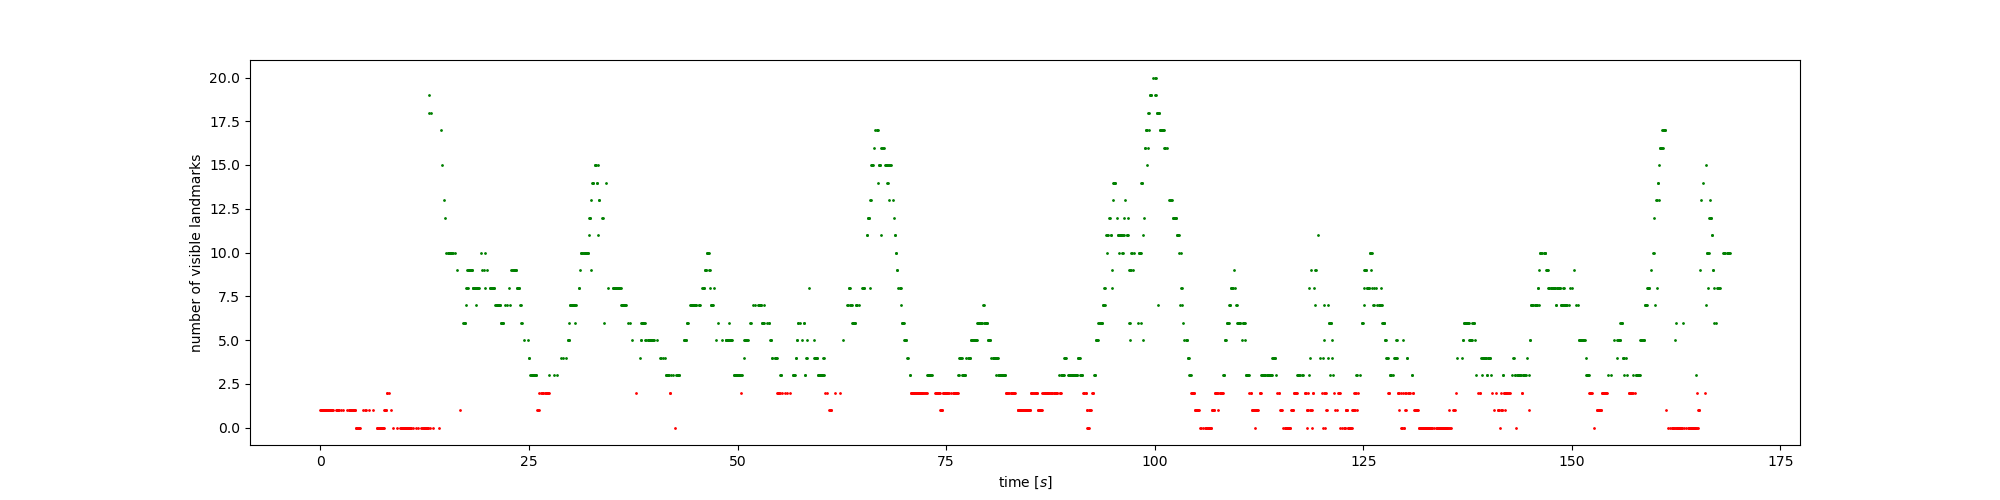
\includegraphics[width=\textwidth]{code/num_visible.png}
    \caption{Number of visible landmarks.}
    \label{fig:4}
\end{figure}

\section*{Question 5}

Several observations can be made regarding the error plots 
\begin{enumerate}
    \item Compare each error plot with plot in question 4, it is obvious that uncertainty is larger at time steps with fewer observations/visible landmarks, as can be seen by the correspondence between spikes of the uncertainty envelopes and frequency of red dots or lower green dots. Specifically, at time steps between the early 130 to 140 where visible landmarks are the fewest, the uncertainty envelopes appear to be the largest over the entire estimation time length.  
    %
    \item The BATCH case has the best accuracy compared to SLIDING WINDOW case, and SLIDING WINDOW with longer window size has better accuracy than the shorter one. It makes sense since BATCH case carries out the full optimization while SLIDING WINDOW cases optimization over each limited time frame, resulting in overall sub-optimality. 
    %
    \item SLIDING WINDOW case has smaller uncertainty envelop than the BATCH case, since each optimization is done over a shorted time length resulting in less uncertainty propagation. 
    %
    \item SLIDING WINDOW cases are more computational efficient than BATCH case, with smaller window size it becomes more efficient as well since the optimization is done over a smaller state space resulting in faster Cholesky decomposition and hence faster linear equation solving for each Newton-Gaussian update step. In practice, since the BATCH case can be properly vectorized it could be faster than SLIDING WINDOWS since SLIDING WINDOW case requires sequential optimization per update step, which might be hard to parallelize due to the initialization dependency and hence slower computation than the BATCH case.  
\end{enumerate}
% Timing of each method (total: including initialization)
% batch:                  60.36846375465393  -> most operations are vectorized so this is fast
% sliding window k = 50:  328.1452748775482
% sliding window k = 10:  49.67981147766113

\begin{figure}[H]
    \centering
    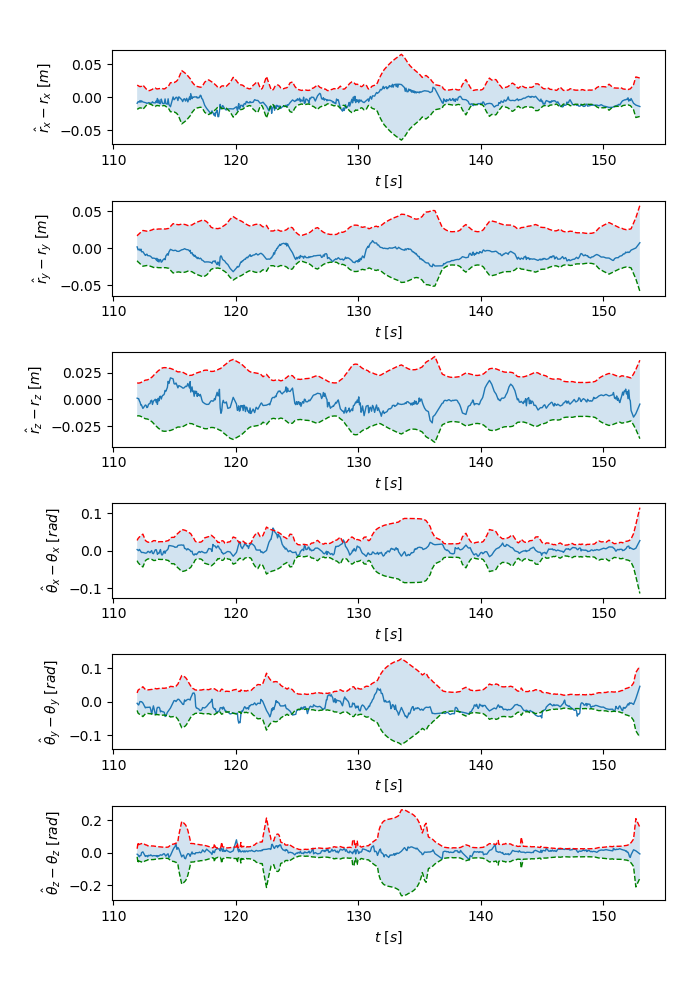
\includegraphics[width=\textwidth]{code/batch.png}
    \caption{Batch optimization}
    \label{fig:5a}
\end{figure}

\begin{figure}[H]
    \centering
    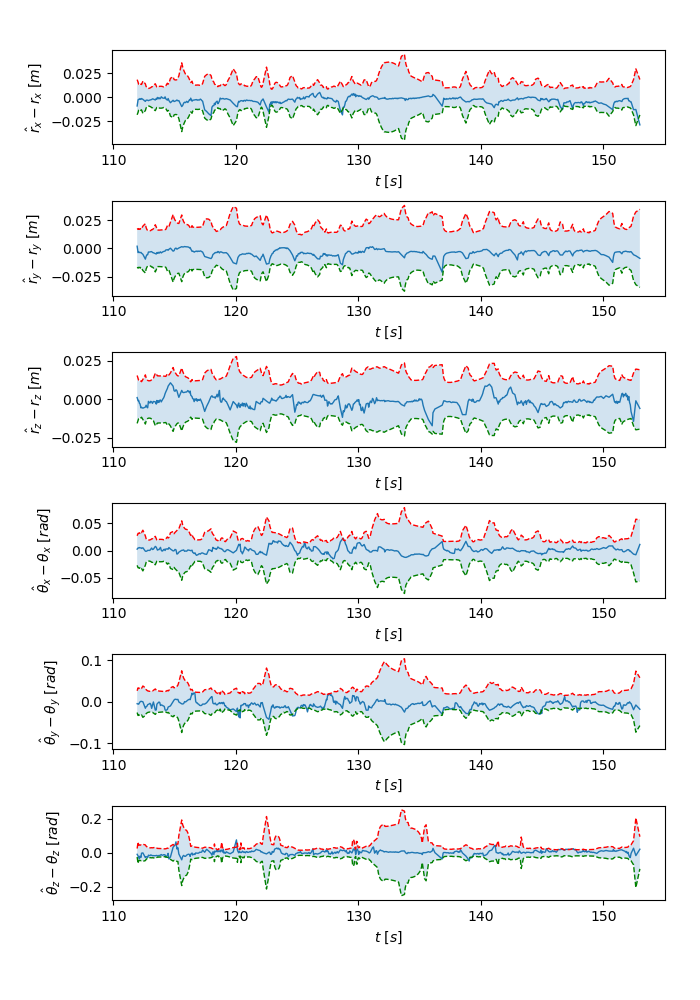
\includegraphics[width=\textwidth]{code/sliding_window_50.png}
    \caption{Sliding window optimization with $\kappa= 50$.}
    \label{fig:5b}
\end{figure}

\begin{figure}[H]
    \centering
    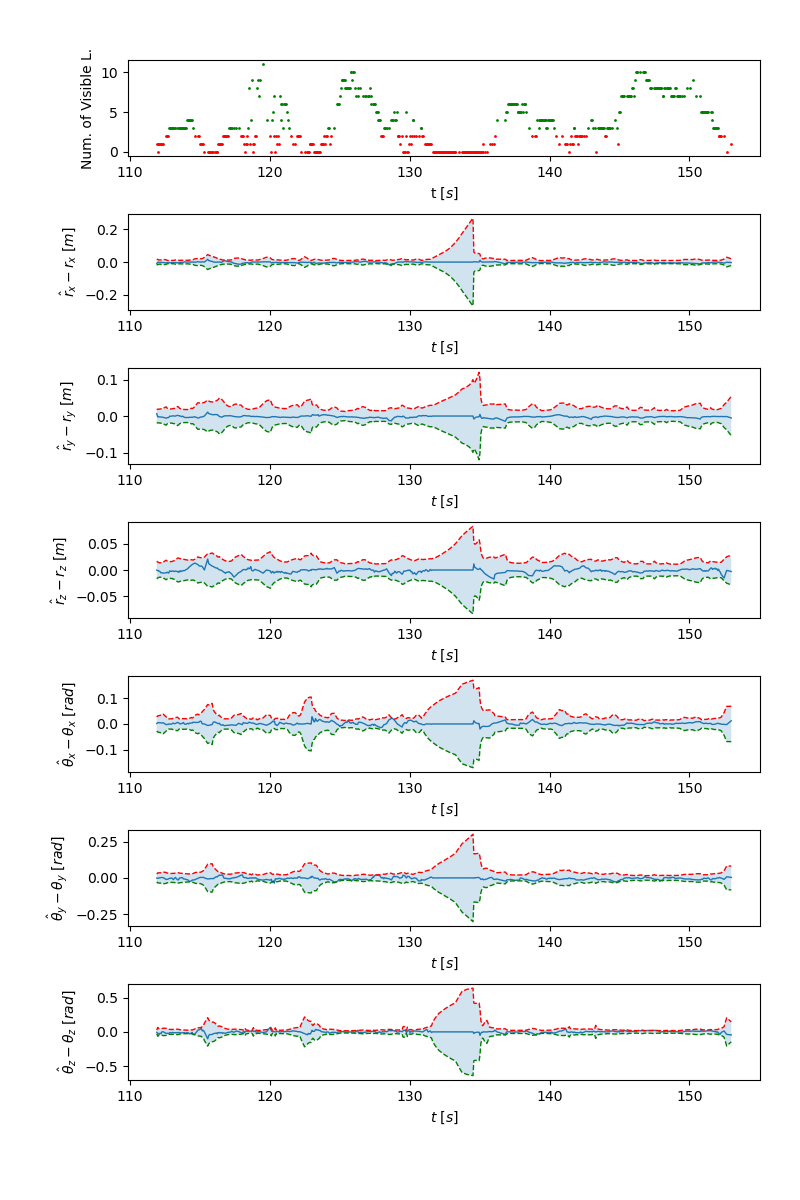
\includegraphics[width=\textwidth]{code/sliding_window_10.png}
    \caption{Sliding window optimization with $\kappa= 10$.}
    \label{fig:5c}
\end{figure}


\clearpage
\printbibliography

\appendix

\clearpage
\section{Source Code}
\label{sourcecode}

\begin{lstlisting}[language=Python, basicstyle=\small, caption=main.py]
import time
import os
import numpy as np
import numpy.linalg as npla
from numpy.linalg import inv
import scipy.linalg as cpla
from scipy.io import loadmat
import matplotlib
import matplotlib.pyplot as plt

import so3
import se3

## Configure matplotlib
matplotlib.use("TkAgg")
matplotlib.rcParams["pdf.fonttype"] = 42
matplotlib.rcParams["ps.fonttype"] = 42
SMALL_SIZE = 10
MEDIUM_SIZE = 12
BIGGER_SIZE = 16
plt.rc("font", size=MEDIUM_SIZE)  # controls default text sizes
plt.rc("figure", titlesize=MEDIUM_SIZE)  # fontsize of the figure title
plt.rc("axes", titlesize=MEDIUM_SIZE)  # fontsize of the axes title
plt.rc("axes", labelsize=SMALL_SIZE)  # fontsize of the x and y labels
plt.rc("xtick", labelsize=SMALL_SIZE)  # fontsize of the tick labels
plt.rc("ytick", labelsize=SMALL_SIZE)  # fontsize of the tick labels
plt.rc("legend", fontsize=SMALL_SIZE)  # legend fontsize


class Estimator:

  def __init__(self, dataset):
    # load data
    data = loadmat(dataset)

    # total time steps
    self.K = data["t"].shape[-1]

    # stereo camera
    self.f_u = data["fu"][0, 0]
    self.f_v = data["fv"][0, 0]
    self.c_u = data["cu"][0, 0]
    self.c_v = data["cv"][0, 0]
    self.b = data["b"][0, 0]

    # stereo camera and imu
    C_c_v, rho_v_c_v = data["C_c_v"], data["rho_v_c_v"]
    self.T_c_v = se3.Cr2T(C_c_v, rho_v_c_v)

    # ground truth values
    r_i_vk_i = data["r_i_vk_i"].T[..., None]
    C_vk_i = so3.psi_to_C(data["theta_vk_i"].T[..., None])
    self.T_vk_i = se3.Cr2T(C_vk_i, r_i_vk_i)  # this is the ground truth

    # inputs
    w_vk_vk_i, v_vk_vk_i = data["w_vk_vk_i"].T, data["v_vk_vk_i"].T
    self.varpi_vk_i_vk = np.concatenate([-v_vk_vk_i, -w_vk_vk_i],
                                        axis=-1)[..., None]
    self.t = data["t"].squeeze()  # time steps (1900,)
    ts = np.roll(self.t, 1)
    ts[0] = 0
    self.dt = self.t - ts

    # measurements
    rho_i_pj_i = data["rho_i_pj_i"].T[
        ..., None]  # feature positions (20 x 3 x 1)
    rho_i_pj_i = np.repeat(rho_i_pj_i[None, ...], self.K,
                           axis=0)  # feature positions (1900, 20 x 3 x 1)
    padding = np.ones(rho_i_pj_i.shape[:-2] + (1,) + rho_i_pj_i.shape[-1:])
    self.rho_i_pj_i = np.concatenate((rho_i_pj_i, padding), axis=-2)
    self.y_k_j = data["y_k_j"].transpose(
        (1, 2, 0))[..., None]  # measurements (1900, 20, 4, 1)
    self.y_filter = np.where(self.y_k_j == -1, 0,
                             1)  # [..., 0, 0] # filter (1900, 20, 4, 1)

    # covariances
    w_var, v_var, y_var = data["w_var"], data["v_var"], data["y_var"]
    w_var_inv = np.reciprocal(w_var.squeeze())
    v_var_inv = np.reciprocal(v_var.squeeze())
    y_var_inv = np.reciprocal(y_var.squeeze())
    self.Q_inv = np.zeros((self.K, 6, 6))
    self.Q_inv[..., :, :] = cpla.block_diag(np.diag(v_var_inv),
                                            np.diag(w_var_inv))
    self.R_inv = np.zeros((*(self.y_k_j.shape[:2]), 4, 4))
    self.R_inv[..., :, :] = np.diag(y_var_inv)

    # helper matrices
    self.D = np.array([[1, 0, 0, 0], [0, 1, 0, 0], [0, 0, 1, 0]])

    # estimated values of variables
    self.hat_T_vk_i = np.zeros_like(self.T_vk_i)
    self.hat_T_vk_i[...] = self.T_vk_i[
        ...]  # estimate of poses initialized to be ground truth
    self.hat_P = np.zeros((self.K, 6, 6))
    self.hat_P[..., :, :] = np.eye(6) * 1e-4
    self.hat_stds = np.ones((self.K, 6)) * np.sqrt(1e-4)
    # copy for initial prior values (opdated by optimize function)
    self.init_T_vk_i = np.zeros_like(self.hat_T_vk_i)
    self.init_T_vk_i[...] = self.hat_T_vk_i[...]
    self.init_P = np.zeros_like(self.hat_P)
    self.init_P[...] = self.hat_P[...]

    self.k1 = 0
    self.k2 = self.K - 1

    # Timing
    self.optimization_time = 0

  def set_interval(self, k1=None, k2=None):
    self.k1 = k1 if k1 != None else self.k1
    self.k2 = k2 if k2 != None else self.k2

  def initialize(self, k1=None, k2=None):
    """
    Initialize a portion of the states between k1 and k2 using dead reckoning
    and starting with the current estimate of k1

    Note: we initialize our estimate with ground truth (hack) in constructor
    call
    """
    k1 = self.k1 if k1 is None else k1
    k2 = self.k2 if k2 is None else k2

    # self.hat_T_vk_i[k1] = self.T_vk_i[k1]  # force to ground truth
    # self.hat_P[k1] = 1e-3 * np.eye(6)      # force to ground truth
    for k in range(k1 + 1, k2 + 1):
      # TODO: need to check initialization, input time step is strange (but same as in assignment)
      # mean
      self.hat_T_vk_i[k] = self.f(self.hat_T_vk_i[k - 1],
                                  self.varpi_vk_i_vk[k - 1], self.dt[k])
      # covariance
      F = self.df(self.hat_T_vk_i[k - 1], self.varpi_vk_i_vk[k - 1],
                  self.dt[k])
      Q_inv = self.Q_inv[k]
      Q_inv = Q_inv / (self.dt[k, None, None]**2)
      self.hat_P[k] = F @ self.hat_P[k - 1] @ F.T + npla.inv(Q_inv)

    # this is only for the initial error term
    self.init_T_vk_i[...] = self.hat_T_vk_i[...]
    self.init_P[...] = self.hat_P[...]

  def optimize(self, k1=None, k2=None):
    k1 = self.k1 if k1 is None else k1
    k2 = self.k2 if k2 is None else k2

    start_time = time.time()

    curr_iter, eps = 0, np.inf
    while curr_iter < 20 and eps > 1e-5:
      eps = self.update(k1, k2)
      curr_iter += 1
      print('GN step: {}   eps: {}'.format(curr_iter, eps))

    self.optimization_time += time.time() - start_time

    # this is only for the initial error term
    self.init_T_vk_i[...] = self.hat_T_vk_i[...]
    self.init_P[...] = self.hat_P[...]

  def update(self, k1=None, k2=None):
    k1 = self.k1 if k1 is None else k1
    k2 = self.k2 if k2 is None else k2

    # First input factor
    # error
    T = self.hat_T_vk_i[k1]
    T_prior = self.init_T_vk_i[k1]
    e_v0 = self.e_v0(T_prior, T)
    # Jacobian
    H_v0 = np.zeros((6, (k2 - k1 + 1) * 6))
    H_v0[:6, :6] = np.eye(6)
    # covariance
    P0_inv = npla.inv(self.init_P[k1])

    # Subsequent input errors
    T = self.hat_T_vk_i[k1:k2]
    T2 = self.hat_T_vk_i[k1 + 1:k2 + 1]
    v = self.varpi_vk_i_vk[k1:k2]
    dt = self.dt[k1 + 1:k2 + 1]
    # error
    e_v = self.e_v(T2, T, v, dt).reshape(-1, 1)
    # Jacobian
    F = self.F(T2, T, v, dt)
    H_v = np.zeros(((k2 - k1) * 6, (k2 - k1 + 1) * 6))
    for i in range(F.shape[0]):
      H_v[6 * i:6 * (i + 1), 6 * i:6 * (i + 1)] = -F[i]
      H_v[6 * i:6 * (i + 1), 6 * (i + 1):6 * (i + 2)] = np.eye(6)
    # covariance
    Q_inv = self.Q_inv[k1 + 1:k2 + 1]
    Q_inv = Q_inv / (dt[..., None, None]**2)
    Q_inv = cpla.block_diag(*Q_inv)

    # Measurement errors
    p = self.rho_i_pj_i[k1:k2 + 1]
    y = self.y_k_j[k1:k2 + 1]
    T = np.repeat(self.hat_T_vk_i[k1:k2 + 1][:, None, ...],
                  self.y_k_j.shape[1],
                  axis=1)
    # error
    e_y = self.e_y(y, p, T).reshape(-1, 1)
    # Jacobian
    G = self.G(y, p, T)
    H_y = np.zeros((np.prod(G.shape[0:3]), (k2 - k1 + 1) * 6))
    nrow = np.prod(G.shape[1:3])
    for i in range(G.shape[0]):
      H_y[nrow * i:nrow * (i + 1), 6 * i:6 * (i + 1)] = G[i].reshape(-1, 6)
    # covariance
    R_inv = self.R_inv[k1:k2 + 1]
    R_inv = R_inv.reshape(-1, 4, 4)
    R_inv = cpla.block_diag(*R_inv)
    # filter out invalid measurements
    mask = self.y_filter[k1:k2 + 1].reshape(-1)
    mask = np.argwhere(mask).squeeze()
    e_y = e_y[mask]
    H_y = H_y[mask]
    R_inv = R_inv[mask][:, mask]

    # Stack all the factors
    e = np.concatenate((e_v0, e_v, e_y), axis=0)
    H = np.concatenate((H_v0, H_v, H_y), axis=0)
    W_inv = cpla.block_diag(P0_inv, Q_inv, R_inv)
    # e = np.concatenate((e_v, e_y), axis = 0)
    # H = np.concatenate((H_v, H_y), axis=0)
    # W_inv = cpla.block_diag(Q_inv, R_inv)

    # Solve the linear system
    LHS = H.T @ W_inv @ H
    RHS = H.T @ W_inv @ e
    update = cpla.cho_solve(cpla.cho_factor(LHS), RHS)
    eps = npla.norm(update)

    # Update each pose
    # mean
    T = self.hat_T_vk_i[k1:k2 + 1]
    update = update.reshape(T.shape[0], 6, 1)
    self.hat_T_vk_i[k1:k2 + 1] = se3.expm(se3.wedge_op(update)) @ T
    # Covariance
    full_hat_P = npla.inv(LHS)
    self.hat_P[k1:k2 + 1] = np.array([
        full_hat_P[i * 6:(i + 1) * 6, i * 6:(i + 1) * 6]
        for i in range(int(full_hat_P.shape[0] / 6))
    ])
    # for plotting
    self.hat_stds[k1:k2 + 1] = (np.sqrt(np.diag(full_hat_P))).reshape(
        (-1, 6))

    return eps

  def plot_trajectory(self, k1=None, k2=None):
    k1 = self.k1 if k1 is None else k1
    k2 = self.k2 if k2 is None else k2

    C_vk_i, r_i_vk_i = se3.T2Cr(self.T_vk_i)
    hat_C_vk_i, hat_r_i_vk_i = se3.T2Cr(self.hat_T_vk_i)

    fig = plt.figure()
    fig.set_size_inches(10, 5)
    ax = fig.add_subplot(111, projection='3d')
    ax.scatter(hat_r_i_vk_i[:, 0],
               hat_r_i_vk_i[:, 1],
               hat_r_i_vk_i[:, 2],
               s=0.1,
               c='blue',
               label='estimate')
    ax.scatter(r_i_vk_i[:, 0],
               r_i_vk_i[:, 1],
               r_i_vk_i[:, 2],
               s=0.1,
               c='blue',
               label='ground truth')
    ax.set_xlabel('x [m]')
    ax.set_ylabel('y [m]')
    ax.set_zlabel('z [m]')
    ax.set_xlim3d(0, 5)
    ax.set_ylim3d(0, 5)
    ax.set_zlim3d(0, 3)
    ax.legend()
    # plt.show()

  def plot_num_visible_landmarks(self):
    num_meas = np.sum(self.y_filter[..., :, 0, 0], axis=-1)
    green = np.argwhere(num_meas >= 3)
    red = np.argwhere(num_meas < 3)

    fig = plt.figure()
    fig.set_size_inches(8, 3)
    fig.subplots_adjust(left=0.1, bottom=0.2)
    ax = fig.add_subplot(111)
    ax.scatter(self.t[green], num_meas[green], s=1, c='green')
    ax.scatter(self.t[red], num_meas[red], s=1, c='red')
    ax.set_xlabel(r't [$s$]')
    ax.set_ylabel(r'Number of Visible Landmarks')
    fig.savefig('num_visible.png')
    # plt.show()

  def plot_error(self, filename, k1=None, k2=None):
    k1 = self.k1 if k1 is None else k1
    k2 = self.k2 if k2 is None else k2

    C_vk_i, r_i_vk_i = se3.T2Cr(self.T_vk_i)
    hat_C_vk_i, hat_r_i_vk_i = se3.T2Cr(self.hat_T_vk_i)

    eye = np.zeros_like(C_vk_i)
    eye[..., :, :] = np.eye(3)
    rot_err = so3.vee_op(eye - hat_C_vk_i @ npla.inv(C_vk_i))
    trans_err = hat_r_i_vk_i - r_i_vk_i

    t = self.t[k1:k2 + 1]
    stds = self.hat_stds[k1:k2 + 1, :]

    # plot landmarks for reference
    num_meas = np.sum(self.y_filter[k1:k2 + 1, :, 0, 0], axis=-1)
    green = np.argwhere(num_meas >= 3)
    red = np.argwhere(num_meas < 3)

    plot_number = 711
    fig = plt.figure()
    fig.set_size_inches(8, 12)
    fig.subplots_adjust(left=0.16,
                        right=0.95,
                        bottom=0.1,
                        top=0.95,
                        wspace=0.7,
                        hspace=0.6)

    plt.subplot(plot_number)
    plt.scatter(t[green], num_meas[green], s=1, c='green')
    plt.scatter(t[red], num_meas[red], s=1, c='red')
    plt.xlabel(r't [$s$]')
    plt.ylabel(r'Num. of Visible L.')

    labels = ['x', 'y', 'z']
    for i in range(3):
      plt.subplot(plot_number + 1 + i)
      plt.plot(t, trans_err[k1:k2 + 1, i].flatten(), '-', linewidth=1.0)
      plt.plot(t, 3 * stds[:, i], 'r--', linewidth=1.0)
      plt.plot(t, -3 * stds[:, i], 'g--', linewidth=1.0)
      plt.fill_between(t, -3 * stds[:, i], 3 * stds[:, i], alpha=0.2)
      plt.xlabel(r"$t$ [$s$]")
      plt.ylabel(r"$\hat{r}_x - r_x$ [$m$]".replace("x", labels[i]))
    for i in range(3):
      plt.subplot(plot_number + 4 + i)
      plt.plot(t, rot_err[k1:k2 + 1, i].flatten(), '-', linewidth=1.0)
      plt.plot(t, 3 * stds[:, 3 + i], 'r--', linewidth=1.0)
      plt.plot(t, -3 * stds[:, 3 + i], 'g--', linewidth=1.0)
      plt.fill_between(t,
                       -3 * stds[:, 3 + i],
                       3 * stds[:, 3 + i],
                       alpha=0.2)
      plt.xlabel(r"$t$ [$s$]")
      plt.ylabel(r"$\hat{\theta}_x - \theta_x$ [$rad$]".replace(
          "x", labels[i]))

    fig.savefig('{}.png'.format(filename))
    # plt.show()
    # plt.close()

  def f(self, T, v, dt):
    """
    Vectorized
    motion model
    """
    dt = dt.reshape(-1, *([1] * len(v.shape[1:])))
    return se3.expm(dt * se3.wedge_op(v)) @ T

  def df(self, T, v, dt):
    """
    Vectorized
    linearized motion model
    """
    dt = dt.reshape(-1, *([1] * len(v.shape[1:])))
    return se3.expm(dt * se3.curly_wedge_op(v))

  def e_v0(self, T_prior, T):
    """
    Vectorized
    initial error
    """
    return se3.vee_op(se3.logm(T_prior @ npla.inv(T)))

  def e_v(self, T2, T, v, dt):
    """
    Vectorized
    the motion error given states at two time steps and input
    """
    return se3.vee_op(se3.logm(self.f(T, v, dt) @ npla.inv(T2)))

  def F(self, T2, T, v, dt):
    """
    Vectorized
    F matrix between two poses
    """
    return se3.Ad(T2 @ npla.inv(T))

  def e_y(self, y, p, T):
    """
    Vectorized
    e matrix measurement
    """
    z = self.D @ self.T_c_v @ T @ p
    g = np.zeros(z.shape[:-2] + (4, 1))
    g[..., 0, 0] = self.f_u * z[..., 0, 0] / z[..., 2, 0] + self.c_u
    g[..., 1, 0] = self.f_u * z[..., 1, 0] / z[..., 2, 0] + self.c_v
    g[..., 2,
      0] = self.f_u * (z[..., 0, 0] - self.b) / z[..., 2, 0] + self.c_u
    g[..., 3, 0] = self.f_u * z[..., 1, 0] / z[..., 2, 0] + self.c_v
    return y - g

  def G(self, y, p, T):
    """
    Vectorized
    G matrix measurement
    """
    z = self.D @ self.T_c_v @ T @ p
    dgdz = np.zeros(z.shape[:-2] + (4, 3))
    dgdz[..., 0, 0] = self.f_u / z[..., 2, 0]
    dgdz[..., 0, 2] = -self.f_u * z[..., 0, 0] / (z[..., 2, 0]**2)
    dgdz[..., 1, 1] = self.f_v / z[..., 2, 0]
    dgdz[..., 1, 2] = -self.f_v * z[..., 1, 0] / (z[..., 2, 0]**2)
    dgdz[..., 2, 0] = self.f_u / z[..., 2, 0]
    dgdz[..., 2,
         2] = -self.f_u * (z[..., 0, 0] - self.b) / (z[..., 2, 0]**2)
    dgdz[..., 3, 1] = self.f_v / z[..., 2, 0]
    dgdz[..., 3, 2] = -self.f_v * z[..., 1, 0] / (z[..., 2, 0]**2)
    dzdx = self.D @ self.T_c_v @ se3.odot_op(T @ p)
    return dgdz @ dzdx


if __name__ == "__main__":

  dataset = "/home/yuchen/Projects/AER1513-A3-Draft/code/dataset3.mat"

  # Plot valid measurements
  print('Q4 Plot valid measurements')
  estimator = Estimator(dataset)
  estimator.plot_num_visible_landmarks()

  # Batch case
  print('Q5(a) batch optimization')
  estimator = Estimator(dataset)
  # start_time = time.time()
  estimator.set_interval(1215, 1714)
  estimator.initialize()  # initialize with odometry
  estimator.optimize()
  batch_time = estimator.optimization_time
  estimator.plot_error("batch")

  print('Q5(b) sliding window optimization with kappa=50')
  k1 = 1215
  k2 = 1714
  kappa = 50
  estimator = Estimator(dataset)
  # start_time = time.time()
  estimator.set_interval(k1, k1 + 50)
  # initialize with odometry using ground truth
  estimator.initialize()
  estimator.optimize()
  for k in range(k1 + 1, k2 + 1):
    print('Current k =', k)
    estimator.set_interval(k, k + 50)
    # initialize with odometry at the previous step
    estimator.initialize(k - 1)
    estimator.optimize()
  sliding_50_time = estimator.optimization_time
  estimator.plot_error("sliding_window_50", k1, k2)

  print('Q5(b) sliding window optimization with kappa=10')
  k1 = 1215
  k2 = 1714
  kappa = 10
  estimator = Estimator(dataset)
  # start_time = time.time()
  estimator.set_interval(k1, k1 + kappa)
  # initialize with odometry using ground truth
  estimator.initialize()
  estimator.optimize()
  for k in range(k1 + 1, k2 + 1):
    print('Current k =', k)
    estimator.set_interval(k, k + kappa)
    # initialize with odometry at the previous step
    estimator.initialize(k - 1)
    estimator.optimize()
  sliding_10_time = estimator.optimization_time
  estimator.plot_error("sliding_window_10", k1, k2)

  print("Timing - ")
  print("batch:                 ", batch_time)
  print("sliding window k = 50: ", sliding_50_time)
  print("sliding window k = 10: ", sliding_10_time)
\end{lstlisting}

\begin{lstlisting}[language=Python, basicstyle=\small, caption=se3.py]
import numpy as np
import numpy.linalg as npla
import scipy.linalg as cpla

import so3


def Cr2T(C_a_b, r_b_a_b):
  """
  Vectorized but not broadcastable
  Rotation matrix and translation vector to pose matrix
    C_{ab}: ...x3x3 matrix
    r_{b}^{ab}: ...x3x1 matrix
  """
  assert C_a_b.shape[:-2] == r_b_a_b.shape[:-2]

  r_a_b_a = -C_a_b @ r_b_a_b
  T_a_b = np.zeros(C_a_b.shape[:-2] + (4, 4))
  T_a_b[..., :3, :3] = C_a_b
  T_a_b[..., :3, 3:4] = r_a_b_a
  T_a_b[..., 3, 3] = 1
  return T_a_b


def T2Cr(T_a_b):
  """
  Vectorized but not broadcastable
  pose matrix to rotation matrix and translation vector 
    T_{ab}: ...x4x4 matrix
  """
  r_a_b_a = T_a_b[..., :3, 3:4]
  C_a_b = T_a_b[..., :3, :3]
  r_b_a_b = -C_a_b.swapaxes(-2, -1) @ r_a_b_a
  return C_a_b, r_b_a_b


def expm(x):
  if len(x.shape) == 2:
    return cpla.expm(x)
  else:
    shape = x.shape
    x = x.reshape(-1, *x.shape[-2:])
    expx = np.zeros_like(x)
    for i in range(x.shape[0]):
      expx[i] = cpla.expm(x[i])
    expx.reshape(shape)
    return expx


def logm(x):
  if len(x.shape) == 2:
    return cpla.logm(x)
  else:
    shape = x.shape
    x = x.reshape(-1, *x.shape[-2:])
    logx = np.zeros_like(x)
    for i in range(x.shape[0]):
      logx[i] = cpla.logm(x[i])
    logx.reshape(shape)
    return logx


def wedge_op(x):
  """
  Vectorized
    x: ...x6x1 vector
  """
  x_wedge = np.zeros(x.shape[:-2] + (4, 4))
  x_wedge[..., :3, :3] = so3.wedge_op(x[..., 3:, :])
  x_wedge[..., :3, 3:4] = x[..., :3, :]
  return x_wedge


def vee_op(x):
  """
  Vectorized
    x: ...x4x4 matrix
  """
  x_vee = np.zeros(x.shape[:-2] + (6, 1))
  x_vee[..., 3:, :] = so3.vee_op(x[..., :3, :3])
  x_vee[..., :3, :] = x[..., :3, 3:4]
  return x_vee


def curly_wedge_op(x):
  """
  Vectorized
    x: ...x6x1 vector
  """
  x_curly_wedge = np.zeros(x.shape[:-2] + (6, 6))
  x_curly_wedge[..., :3, :3] = so3.wedge_op(x[..., 3:, :])
  x_curly_wedge[..., 3:, 3:] = so3.wedge_op(x[..., 3:, :])
  x_curly_wedge[..., :3, 3:] = so3.wedge_op(x[..., :3, :])
  return x_curly_wedge


def odot_op(p):
  """
  Vectorized
    p: ...x4x1 vector
  """
  eye = np.zeros(p.shape[:-2] + (3, 3))
  eye[..., :, :] = np.eye(3)
  eps = p[..., :-1, :]
  eta = p[..., 3, 0]
  eta = eta.reshape(*eta.shape, *([1] * len(eye.shape[-2:])))
  p_odot = np.zeros(p.shape[:-2] + (4, 6))
  p_odot[..., :3, :3] = eta * eye
  p_odot[..., :3, 3:] = -so3.wedge_op(eps)
  return p_odot


def Ad(T):
  Ad_T = np.zeros(T.shape[:-2] + (6, 6))
  C = T[..., :3, :3]
  r = T[..., :3, 3:4]
  Ad_T[..., :3, :3] = C
  Ad_T[..., 3:, 3:] = C
  Ad_T[..., :3, 3:] = so3.cross_op(r) @ C
  return Ad_T


if __name__ == "__main__":
  # test Cr2T
  C = np.zeros((5, 4, 3, 3))
  r = np.zeros((5, 4, 3, 1))
  T = Cr2T(C, r)
  C = np.zeros((3, 3))
  r = np.zeros((3, 1))
  T = Cr2T(C, r)
  print(T)
\end{lstlisting}

\begin{lstlisting}[language=Python, basicstyle=\small, caption=so3.py]
import numpy as np
import numpy.linalg as npla


def cross_op(x):
  """
  Vectorized
  compute x^cross, the skew symmetric matrix
    x: ...x3x1 vector
  """
  x_cross = np.zeros(x.shape[:-2] + (3, 3))
  x_cross[..., 0, 1] = -x[..., 2, 0]
  x_cross[..., 0, 2] = x[..., 1, 0]
  x_cross[..., 1, 0] = x[..., 2, 0]
  x_cross[..., 1, 2] = -x[..., 0, 0]
  x_cross[..., 2, 0] = -x[..., 1, 0]
  x_cross[..., 2, 1] = x[..., 0, 0]
  return x_cross


def wedge_op(x):
  return cross_op(x)


def vee_op(x):
  x_vee = np.zeros(x.shape[:-2] + (3, 1))
  x_vee[..., 0, 0] = x[..., 2, 1]
  x_vee[..., 1, 0] = x[..., 0, 2]
  x_vee[..., 2, 0] = x[..., 1, 0]
  return x_vee


def psi_to_C(psi):
  """
  Vectorized
  axis angle to rotation matrix
    psi: ...x3x1 vector
  """
  ag = npla.norm(psi, axis=(-2, -1), keepdims=True)
  ax = psi / ag
  eye = np.zeros(ag.shape[:-2] + (3, 3))
  eye[..., :, :] = np.eye(3)
  C = np.cos(ag) * eye + (1 - np.cos(ag)) * (
      ax @ ax.swapaxes(-2, -1)) - np.sin(ag) * cross_op(ax)
  return C
\end{lstlisting}

\end{document}
